\section{Форматы данных}

Объектная модель события представляет данные в программе,
в то время как задачу хранения данных нужно решать с
привлечением различных стандартизированных средств.

Коротко рассмотрим реализации кодировщиков моделей события
и выходных данных.

\subsection{Форматы хранения событий}

Использование различных форматов хранения данных в программном окружении
является одним из основных предметов модульной архитектуры.
Благодаря средствам статического полиморфизма поддержка
различных форматов выполняется в виде шаблонных
специализаций, основанных на шаблонном обходе топологии типов.

Для представления данных о событии применялись следующие форматы:
\begin{itemize}
    \item ROOT \texttt{TTree}, как основной формат принятый
    в экспериментальной физике высоких энергий,
    \item Apache Avro~\cite{avro-spec}, компактный и быстрый
    формат обмена иерархическими
    данными со статической типизацией.
\end{itemize}

Также применялись форматы HDF5~\cite{hdf5-std},
и Google Protocol Buffers~\cite{protobuf-spec}. Хотя их использование
в NA64 прекратилось, для указания на универсальность подхода следует отметить,
что интеграция с ними
осуществлялась в той же парадигме автоматического выведения
реализации на основе статического полиморфизма.

На рисунке~\ref{fig:data-sources-example} приведена диаграмма
классов содержащая пример модульной системы на основе
абстрактных классов \texttt{AbstractDataSource} и
\texttt{AbstractEventHandler}.
%Компоненты интегрирующие
%Apache Avro или предоставляющие источник данных COMPASS DAQ
%могут отсутствовать в системе

\begin{figure}
    \centering
    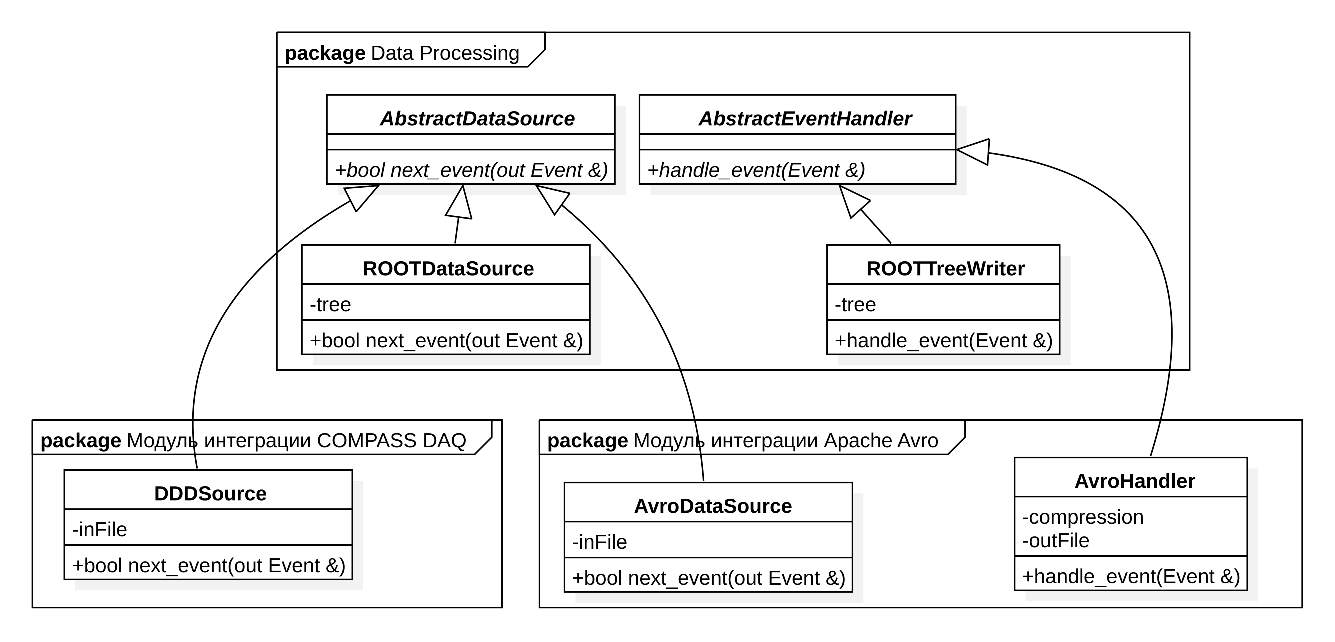
\includegraphics[width=0.95\linewidth]{images/illustrative/data-sources-example.eps}
    \caption{Диаграмма классов иллюстрирующая отношения классов реализующих различные форматы хранения событий}
    \label{fig:data-sources-example}
\end{figure}

Как и в случае с объектной моделью события, рассмотренной ранее,
автоматическая генерация декодировщиков данных относится преимущественно
к внутренним протоколам программного окружения. Интеграция с внешними
источниками осуществляется через отдельные модули,
требующими участия разработчика для сопровождения.

Так, в частности, важнейшим источником является декодирование данных,
считанных напрямую из системы сбора данных (DAQ), которое опирается
на библиотеку кодирования COMPASS~\cite{compass-daq}.

Таким образом, модуль реализующий интерфейс источника данных обычно
является промежуточным слоем между библиотекой и ядром системы.

\subsection{Иерархия детекторов в выходных данных}

Класс \texttt{TDirAdapter} (из окружения ROOT) предоставляет
часто используемые операционные примитивы при отображении
множества детекторов в связанный
набор экземпляров подкласса \texttt{TObject} допускающих
хранение внутри \texttt{TDirectory}. В таком виде удобно
размещать большие наборы гистограмм и
графиков соответствующих индивидуальным детекторам в рамках одного
обработчика. Так, например, с применением идентификаторов детектора,
наглядную иерархию объектов отвечающую
логической структуре детектора изображённую на
рисунке~\ref{fig:tobject-hierarchy} можно получить подстановкой
семантических элементов идентификатора в простой текстовый шаблон.

\begin{figure}
    \centering
    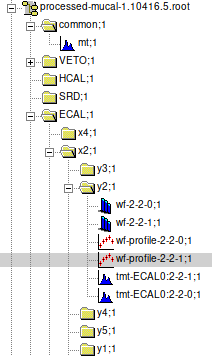
\includegraphics[width=0.25\linewidth]{images//illustrative/items-structure-in-root-file.png}
    \caption{Иерархия объектов внутри \texttt{TFile} порождаемая
    идентификатором детектора на основе шаблонных путей}
    \label{fig:tobject-hierarchy}
\end{figure}

Обработчики включающие \texttt{TDirAdapter} обычно
предусматривают переопределение шаблонов путей для адаптации к
конкретным пользовательским приложениям в тех случаях когда
спецификация входного файла каким-то образом ограничена.

\subsection{Извлечение характеристик распределений}

Например, часто возникающая практическая задача отыскания
коэффициентов распределений на основе особенностей различных
спектров может быть обусловлена в виде короткого конфигурационного
файла задающего:
\begin{itemize}
    \item Шаблон имени гистограммы при помощи регулярных
    выражений с именованными группами захвата для извлечения
    имени детектора и индекса элемента,
    \item Обозначения особенности на
    спектре -- например <<первый минимум по порядку>>,
    <<второй максимум по высоте>>.
\end{itemize}

\begin{figure}
    \centering
    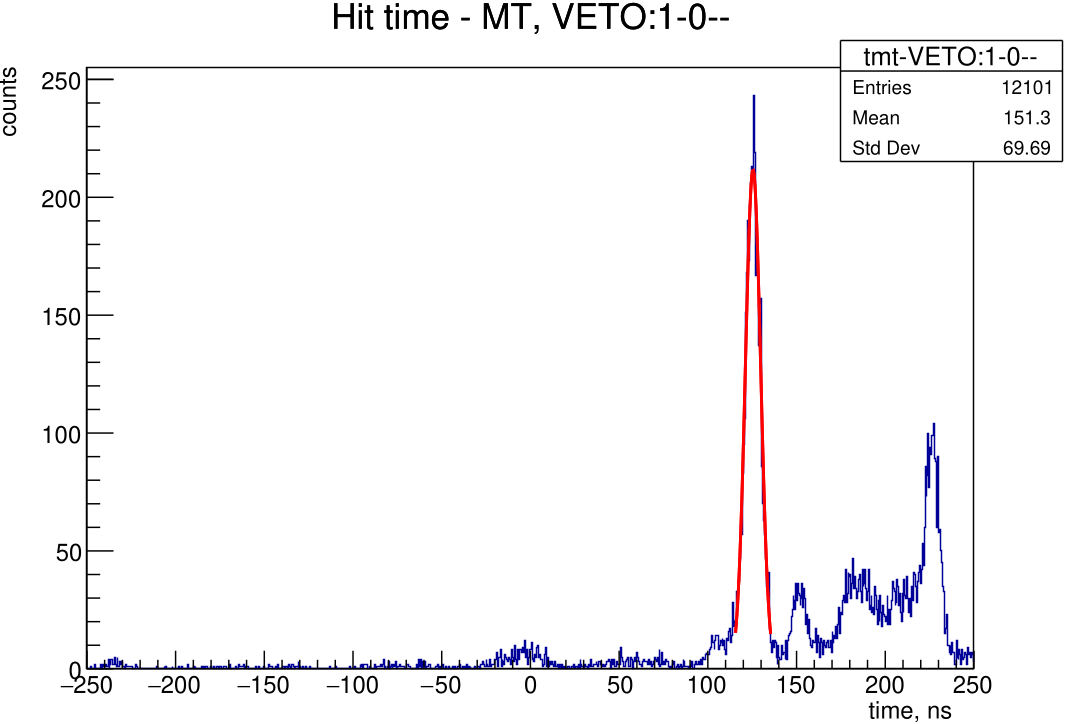
\includegraphics[width=0.5\linewidth]{images//illustrative/tmt-fit-example.png}
    \caption{Пример автоматического выделения основного пика во временном
    распределении мюонного сигнала в вето-детекторе}
    \label{fig:placeholder}
\end{figure}

Обобщение практики применения таких процедур показывает, что количество
особенностей сравнительно невелико, и в большинстве случаев логика,
необходимая для калибровки или автоматизированного анализа, может быть
задана в виде компактной спецификации.
